\documentclass{tufte-handout}

\input{vc.tex}  % For version control

\usepackage{geometry}                % See geometry.pdf to learn the layout options. There are lots.
\geometry{letterpaper}                   % ... or a4paper or a5paper or ... 
%\geometry{landscape}                % Activate for for rotated page geometry
%\usepackage[parfill]{parskip}    % Activate to begin paragraphs with an empty line rather than an indent
\usepackage{tikz}
\usetikzlibrary{decorations.pathmorphing}
\usetikzlibrary{shapes.symbols}
\usetikzlibrary{chains} 
\usetikzlibrary{positioning} 
\usetikzlibrary{calc} 
\usetikzlibrary{decorations.pathreplacing} 
\tikzset{
  vertex/.style = {
    circle,draw, fill = white, inner sep = 0pt, minimum width = 4pt  }
}
\DeclareGraphicsRule{.tif}{png}{.png}{`convert #1 `dirname #1`/`basename #1 .tif`.png}

\usepackage{graphicx}
\usepackage{amssymb}
\usepackage{epstopdf}
\DeclareGraphicsRule{.tif}{png}{.png}{`convert #1 `dirname #1`/`basename #1 .tif`.png}

\title{Rainbow Perfect Matchings}
\author{}
\date{\GITAuthorDate, rev. \GITAbrHash}

\begin{document}
\maketitle
%\section{}
%\subsection{}
\section*{Instructions}
In this home assignment you are going to put together an algorithm yourself. In the previous labs you were given the complete algorithms. Here you will instead be presented with two pieces of the algorithm and it is up to you to assemble it. The idea is to mimic the behavior of an algorithm researcher/engineer. This is no doubt tougher than the labs and it is recommended that you read the whole home assignment and the related material listed in the end \emph{several times} before you actually get to work.

\section*{Description}
\noindent The Rainbow Perfect Matching problem (RPM) is the following: 

You are given a multigraph $G=(V,E)$ with $|V|=2n$, i.e. a graph in which there may be multiple copies of an edge $u,v$ for any pair $u\neq v\in V$. In addition, each edge $e\in E$ has a color $c(e)\in [n]$. The question is whether there exists a \emph{rainbow} perfect matching in $G$, i.e. a subset of the edge $E'\subseteq E$ such that
\begin{itemize}
\item Each vertex in $V$ is the endpoint of exactly one edge in $E'$.
\item There is exactly one edge in $E'$ of every color.
\end{itemize}

\begin{marginfigure}
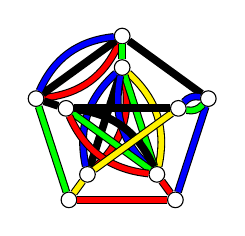
\begin{tikzpicture}[scale=.5,
vertex_style/.style={draw,circle,inner sep=2pt},
edge_style/.style={double = black}]

\begin{scope}[rotate=90]
\foreach \x/\y in {0/1,72/2,144/3,216/4,288/5}{
 \node[vertex_style] (\y) at (canvas polar cs: radius=1.5cm,angle=\x){};
}
\foreach \x/\y in {0/6,72/7,144/8,216/9,288/10}{
 \node[vertex_style] (\y) at (canvas polar cs: radius=2.3cm,angle=\x){};
}
\end{scope}

\begin{scope}[double distance=2pt]

\draw[double = red] (1) to [bend left] (3);
\draw[double = black] (1) -- (3);
\draw[double = blue] (1) to [bend right] (3);

\draw[double = yellow] (1) to [bend left] (4);
\draw[double = green] (1) -- (4);
\draw[double = blue] (1) to [bend right] (4);

\draw[double = black] (2) to [bend left] (4);
\draw[double = green] (2) -- (4);
\draw[double = red] (2) to [bend right] (4);

\draw[double = yellow] (3) -- (5);
\draw[double = black] (5) -- (2);

\draw[double = red] (6) to [bend left] (7);
\draw[double = black] (6) -- (7);
\draw[double = blue] (6) to [bend right] (7);

\draw[double = green] (7) -- (8);
\draw[double = red] (8) -- (9);
\draw[double = blue] (9) -- (10);
\draw[double = black] (10) -- (6);

\draw[double = green] (1) -- (6);
\draw[double = black] (2) -- (7);
\draw[double = yellow] (3) -- (8);
\draw[double = red] (4) -- (9);

\draw[double = blue] (5) to [bend left] (10);
\draw[double = green] (5) to [bend right] (10);
\end{scope}
\end{tikzpicture}
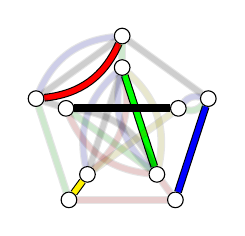
\begin{tikzpicture}[scale=.5,
vertex_style/.style={draw,circle,inner sep=2pt},
edge_style/.style={double = black}]
%\useasboundingbox (-5.05,-4.4) rectangle (5.1,5.25);
\begin{scope}[rotate=90]
\foreach \x/\y in {0/1,72/2,144/3,216/4,288/5}{
 \node[vertex_style] (\y) at (canvas polar cs: radius=1.5cm,angle=\x){};
}
\foreach \x/\y in {0/6,72/7,144/8,216/9,288/10}{
 \node[vertex_style] (\y) at (canvas polar cs: radius=2.3cm,angle=\x){};
}
\end{scope}

%\draw[double = green] (1) -- (4);
%\draw[double = black] (5) -- (2);
%\draw[double = red] (6) -- (7);
%\draw[double = blue] (9) -- (10);
%\draw[double = yellow] (3) -- (8);

\begin{scope}[double distance=2pt, very nearly transparent]

\draw[ double = red] (1) to [bend left] (3);
\draw[ double = black] (1) -- (3);
\draw[ double = blue] (1) to [bend right] (3);

\draw[ double = yellow] (1) to [bend left] (4);
\draw[opaque, double = green] (1) -- (4);
\draw[ double = blue] (1) to [bend right] (4);

\draw[ double = black] (2) to [bend left] (4);
\draw[double = green] (2) -- (4);
\draw[double = red] (2) to [bend right] (4);

\draw[ double = yellow] (3) -- (5);
\draw[opaque,double = black] (5) -- (2);

\draw[opaque,double = red] (6) to [bend left] (7);
\draw[ double = black] (6) -- (7);
\draw[double = blue] (6) to [bend right] (7);

\draw[ double = green] (7) -- (8);
\draw[double = red] (8) -- (9);
\draw[opaque,double = blue] (9) -- (10);
\draw[ double = black] (10) -- (6);

\draw[ double = green] (1) -- (6);
\draw[double = black] (2) -- (7);
\draw[opaque,double = yellow] (3) -- (8);
\draw[ double = red] (4) -- (9);

\draw[ double = blue] (5) to [bend left] (10);
\draw[ double = green] (5) to [bend right] (10);
\end{scope}

%\foreach \x/\y in {6/7,7/8,8/9,9/10,10/6}{
% \draw[edge_style] (\x) -- (\y);
%}
\end{tikzpicture}
\caption{ 
Left: An instance to the RPM problem. Right: A solution to the same instance.
}
\end{marginfigure}

Your task is to come up with an algorithm for a \emph{restricted} version of RPM: We define bRPM as the RPM problem on \emph{balanced bipartite} graphs, i.e. when we know that $V$ can be partitioned in two equal halfs $V_1$ and $V_2$ such that every edge $e\in E$ has one endpoint in $V_1$ and the other in $V_2$.\footnote{Once you
have found the algorithm for bRPM it is not too difficult to modify your algorithm to work for the general RPM. You'll need to exchange the biadjacency matrix for something else but similar. This is however not part of the assignment.}

\begin{marginfigure}
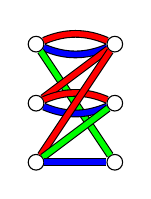
\begin{tikzpicture}[yscale=.75,every node/.style={draw,circle,inner sep=2pt}]
\node (a) at (0,0) {};
\node (b) at (0,-1) {};
\node (c) at (0,-2) {};
\node (1) at (1,0) {};
\node (2) at (1,-1) {};
\node (3) at (1,-2) {};
\begin{scope}[double distance=2pt]
\draw [double = red] (a) to[bend left] (1);
\draw [double = blue] (a) to[bend right] (1);
\draw [double = green] (a) -- (3);
\draw [double = red] (b) -- (1);
\draw [double = red] (b) to [bend left] (2);
\draw [double = blue] (b) to [bend right] (2);
\draw [double = red] (c) -- (1);
\draw [double = green] (c) -- (2);
\draw [double = blue] (c) -- (3);
\end{scope}
\end{tikzpicture}
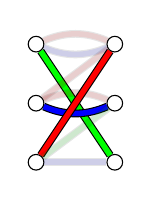
\begin{tikzpicture}[yscale=.75,every node/.style={draw,circle,inner sep=2pt}]
\node (a) at (0,0) {};
\node (b) at (0,-1) {};
\node (c) at (0,-2) {};
\node (1) at (1,0) {};
\node (2) at (1,-1) {};
\node (3) at (1,-2) {};
\begin{scope}[double distance=2pt, very nearly transparent]
\draw [double = red] (a) to[bend left] (1);
\draw [double = blue] (a) to[bend right] (1);
\draw [opaque,double = green] (a) -- (3);
\draw [double = red] (b) -- (1);
\draw [double = red] (b) to [bend left] (2);
\draw [opaque,double = blue] (b) to [bend right] (2);
\draw [opaque,double = red] (c) -- (1);
\draw [double = green] (c) -- (2);
\draw [double = blue] (c) -- (3);
\end{scope}
\end{tikzpicture}
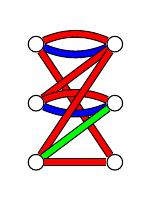
\begin{tikzpicture}[yscale=.75,every node/.style={draw,circle,inner sep=2pt}]
\node (a) at (0,0) {};
\node (b) at (0,-1) {};
\node (c) at (0,-2) {};
\node (1) at (1,0) {};
\node (2) at (1,-1) {};
\node (3) at (1,-2) {};
\begin{scope}[double distance=2pt]
\draw [double = red] (a) to[bend left] (1);
\draw [double = blue] (a) to[bend right] (1);
\draw [double = red] (a) -- (3);
\draw [double = red] (b) -- (1);
\draw [double = red] (b) to [bend left] (2);
\draw [double = blue] (b) to [bend right] (2);
\draw [double = red] (c) -- (1);
\draw [double = green] (c) -- (2);
\draw [double = red] (c) -- (3);
\end{scope}
\end{tikzpicture}
\caption{Left: A bipartite multigraph with coloured edges. Middle: A rainbow perfect
  matching. Right: A graph without a rainbow perfect matching.}
\end{marginfigure}


The bRPM problem is an NP-complete problem, which follows by an easy
reduction from 3-Dimensional Perfect Matching ((8.20) in Kleinberg and
Tardos). Thus, you should expect to end up with an exponential time algorithm.
Below are the descriptions of the two pieces.

\subsection*{Algorithmic Piece 1}
bRPM generalizes ordinary bipartite graph perfect matching: Given a bipartite graph find out if there is a subset of the edges such that every vertex is part of precisely one of the chosen edges. In class (lecture 8, see also [S11] in the related material section at the end of this assignment) we learned how to solve for bipartite perfect matchings with an algebraic technique. We reiterate it here in a slightly modified variant without the use of  fields of characteristic two. We anticipate that you probably will find the version below easier to implement:

 The following algorithm decides if a bipartite graph $G$ contains a
 perfect matching:
\begin{enumerate}
\item Fix a prime $p>\!\!\!>n$.
\item In the biadjacency matrix $A_G$ of the graph $G$, replace each $1$ with a random value between $0$ and $p$. Make your random choices uniformly and independently at random.
\item Compute $m_G=\mbox{det}(A_G)\mbox{ (mod $p$)}$.
\item If $m_G\neq 0$ return ``yes'' else return ``no''.
\end{enumerate}

The idea behind the algorithm is that $m_G$ actually computes a polynomial in edge ``variables'', here replaced by random values, such that there is precisely one monomial in the polynomial for each perfect matching in the graph. The success guarantee is given directly by the Schwartz-Zippel lemma.

\subsection*{Algorithmic Piece 2}
Suppose we had some efficient means to actually \emph{count} the
number of perfect matchings in a bipartite multigraph (no colors
here), then we could use the technique of inclusion--exclusion
(lecture 4, see also [Hu11] in the related material section at the end
of this assignment) to count the rainbow perfect matchings in a bRPM
instance. To see how, let $pm(G)$ for a
bipartite (uncolored) multigraph $G$ be the number of perfect
matchings in $G$.

 The following algorithm computes the number of rainbow perfect matchings in the input bRPM given by the graph $G$ and a
color function $c:E\rightarrow [n]$:

\begin{enumerate}
\item Set $\mbox{sum}=0$.
\item For each $X\subseteq [n]$.
\item \hspace{5mm} Set $G_X=(V_1,V_2,E_X)$ where $E_X=\{e|e\in E, c(e)\in X\}$.
\item \hspace{5mm} $\mbox{sum}=\mbox{sum}+(-1)^{n-|X|}pm(G_X)$.
\item end
\item return \mbox{sum}.
\end{enumerate}

The reason it works is that perfect matchings that do not use all colors, and hence necessarily use some color multiple times, will be counted an even number of times. Exactly half of them will be multiplied with the sign factor $-1$, so they will cancel each other. Formally, if the colors used by the perfect matching $m$ is $C\subset [n]$, we will count the perfect matching $m$ in $pm(G_X)$ for every $X\supseteq C$. For every such $X$ for which $n-|X|$ is odd, we will subtract the matching. But for every $X$ for which $n-|X|$ is even, we will add the matching. Altogether we will get a net result of zero from the matching since there are as many odd sized $X$'s as even sized ones in the set  $\{X|C\subseteq X \subseteq [n]\}$. Rainbow perfect matchings on the other hand, will only be counted once, in $pm(G_{[n]})$.

\bigskip
Unfortunately, we don't have any efficient algorithms to count the number of perfect matchings, but we \emph{do} have algorithmic piece 1.  We need to replace $pm(G)$ for something else that accounts for all perfect matchings in $G$. We will not be able to count the number of rainbow perfect matchings, but we will be able to detect if there is one.

\noindent \emph{Hint: the resulting algorithm should use one ``variable'' for each colored edge in the input bRPM above}.

\section*{Deliverables}
\subsection*{Algorithm description}
Describe in pseudo code how the two algorithmic pieces can be combined into an algorithm for bRPM.
\subsection*{Runtime bound}
Derive the runtime bound in $O(.)$ notation in terms of $n$.
\subsection*{Failure bound}
Present an upper bound on the probability that the algorithm fails to report a solution to a bRPM instance that has a solution.
\subsection*{Implementation}
Implement the algorithm in a programming language of your choice. The trickiest part is probably to compute the determinants. Note that you can \emph{not} use Matlab's det and take the answer modulo the prime $p$ since the internal calculations may overflow. You need to implement a determinant algorithm.
In the appendix we present such an implementation of a determinant mod p function in Matlab.
Use a prime $p$ such that $p^2<2^{30}$. That way you can represent elements and count with them using a standard 32bit \textbf{int} datatype.

\subsection*{Benchmark}
Construct some small instances of the bRBM and test your implementation. Use as large $n$ as you seem fit with respect to the running time. The algorithm should finish in a few seconds for the largest $n$.  Try to make interesting instances that have no solutions as well as instances in which you plant a solution. Test the behavior with respect to the choice of $p$. If you make the prime $p$ just above $n$, say $\approx 2n$,  you should be getting false negatives quite easily.

\section*{Related Material}
\noindent [S11] http://www.cs.berkeley.edu/\textasciitilde sinclair/cs271/n2.pdf

\noindent [Hu11] http://arxiv.org/abs/1105.2942

\end{document}  
